% --------------------------------------------------
% Testing and Validation
% --------------------------------------------------
\chapter{Testing: Verification and Validation}

% Here you explain your approach to testing and show your results. Testing should be a directed process and so there should be some discussion of why you have done the tests you have and why they are appropriate to the validation of your problem solution. You should also consider the limits to your presented verification and validation.

As this project has a lot of moving parts to it, testing is a necessary requirement to ensure how well the objectives stated in Chapter \ref{chapter:probart} have been met and how robust the system is generally.

Testing of the actual code that composes the system was done primarily with the Jest testing framework \cite{jest}

\section{Usability Testing}

% go through all the functionality of the site and tabulate the results

Usability testing is the process of making sure the features that have been implemented are all working by going through them one by one and assessing their performance and quality.

\begin{table}[h]
    \centering
    \begin{tabulary}{\textwidth}{l|C}
        \textbf{Feature} & \textbf{Usability Summary}\\
        \hline
        Monaco Text Editor & Feature works fully with syntax colouring, auto complete with JavaScript but not other languages\\
        \hline
        Code Execution & Fully functioning in all areas that are applicable\\
        \hline
        Terminal Emulator & Performs task well with input and output link issue with small level of latency where the messages are being buffered to only send every 10ms, leads to skipping some characters\\
        \hline
        File browsing & Opening a file and saving to it works, issue where folders aren't displayed correctly\\
        \hline
        Doing an exercise & Works, would be good for code validation to make sure the exercise output is correct but functionally works well\\
        \hline
        Creating an exercise & Works well, currently C exercises can't be made due to the lack of C REPL available\\
        \hline
        Sandbox Page & Would be good to have a run button like in the exercise page, also an issue with resizing windows going off the page\\
        \hline
        Home Page & Would be nice if any code written in the windows was reloaded when the tab to switch language is pressed rather than just putting the default comment in.\\
    \end{tabulary}
\end{table}


% Code editing experience - v good

% Terminal emulator - some latency but not a deal breaker

% Run button on the sandbox page

% Nice having access to bash in the browser

% Expert mode idea for either the REPL or the bash Terminal

% Design - quite good

% Resizing windows - helpful

% Actually validate exercise output

% Error boundaries, react

% Error on homepage for when syntax is invalid etc

\section{Compatibility}

% TODO: use browser stack to make sure the website isn't shit on safari, Edge and opera. Will also need to add media query to show that the editor doesn't work on mobile.

Although web applications don't have to worry about the metal of the system that the browser is relying on, several browsers use different engines and processors in order to render DOM elements to the screen. This means it's good practice to ensure the web application being developed is functional on the different popular and modern browsers.

\begin{table}[h]
    \centering
    \begin{tabulary}{\textwidth}{l|C|c}
        \textbf{Browser} & \textbf{UI Compatibility} & \textbf{Functionality Compatibility} \\
        \hline
        Google Chrome & Fully compatible & Fully compatible \\
        \hline
        Mozilla Firefox & Mostly compatible, only noticeable glitch is the page gains padding when the Monaco auto complete appears & Fully compatible \\
        \hline
        Microsoft Edge & Partially compatible, strange squashing of nav bar component & Fully compatible \\
        \hline
        Apple Safari & Mostly compatible, some scaling issues with text & Fully compatible \\
        \hline
        Internet Explorer 11 & Not compatible, the web app uses CSS Grid for page layout which is not supported in IE 11 & Un-testable
    \end{tabulary}
\end{table}

It's worth noting that Google Chrome's engine, Chromium is now powering a canary build of Microsoft Edge and is already powering Opera, this means that websites that are compatible with Chrome will be equally compatible with these browsers.  

Internet Explorer 11, while having the second highest market share of browsers \cite{browser-stats} is still only 9.83\% with Firefox close behind at 9.62\%. Overall coverage of the application is 84.83\% of all browsers which is a significant volume of users.

Adding support for IE 11 is an option for the future however, considering Microsoft are pushing their Edge browser over IE it isn't a high priority. Most of the usage will be front enterprise machines which can't run latest versions of OS's or web browsers due to security concerns.

This compatibility test didn't test mobile devices as they aren't supported by the Monaco editor so for now a landing page is rendered saying that mobile support is coming.

\section{Code}

Testing code is a way of making sure that the end product that is created is robust to future change. Code testing can come in many forms but this project has focused on \textbf{Unit Testing}.

\subsection{Unit Testing}

Unit testing is the method of testing a component of the system as though it is a completely isolated module a benefit of this is that when writing unit tests themselves it can reveal that code that was previously thought to be modular is not. 

Testing complex functionality is a high priority when thinking about writing unit tests, the WebSocket receiver functionality of the frontend is a good nomination for a test suite as it has many different outputs depending on the WebSocket event received. It also opens up the idea of Test Driven Development because if a new feature is being developed that would involve a new WebSocket event to be received, the event can be mocked (shown in Snippet \ref{snip:socket-test}) and the expected output can be defined. From this starting point the test will fail and the functionality can be added to the \texttt{switch statement} so that the test passes.

\begin{sexylisting}[label=snip:socket-test]{Test for Receiving Container.Start Message}
const MOCK_STATE = {};

test('Container Start', () => {
    const MOCK_EVENT = makeEvent(
        MessageTypes.CONTAINER_START, {
            name: 'Tester',
            info: { Config: { Hostname: 'Tester' } }
        });

    expect(handleMessage(MOCK_EVENT, MOCK_STATE))
        .toMatchSnapshot();

    const TEMP_STATE = { containerName: '', id: '' };

    expect(handleMessage(MOCK_EVENT, TEMP_STATE))
        .toMatchSnapshot();
});
\end{sexylisting}

This test is checking to see if, when a mock event is passed to the function that handles the message, the output is correct and matches the previous snapshot. If the output changes (because the function changes) then this test will fail.

The backend of the application can be tested in a very similar way by mocking inputs and snapshotting outputs, functions can be tested in a way that means they are robust to future change in the codebase so any changes that are unexpected will cause the test to fails.

\section{Performance}

% Lighthouse tests blah blah blah 
Performance testing is making sure that the system is working in an acceptably fast way. Measuring the performance of the front end is done by using the built in Lighthouse tool in Google Chrome and for the backend, as it is famously difficult to measure Docker performance \cite{docker-perf} the measuring will be done locally with the Docker CLI \texttt{docker stats} command which provides real time information on the consumption of the containers that are running.

\subsection{Lighthouse Audits}

Built into Google Chrome is a website auditing tool called \textit{Lighthouse} \cite{google-lighthouse} which can measure many different aspects of web applications such as their performance, search engine optimisation, accessibility, and best practices. 

\textbf{Performance} is focused on things like the first meaningful paint to the screen and how quickly the web page is able to be interacted with. 

\textbf{Search Engine Optimisation (SEO)} is simulating how well a web crawler can crawl through the page and generate a site map so the pages are visible on a search engine. 

\textbf{Accessibility} measures important aspects such as if screen readers can interpret the elements on the page and if any colours aren't contrasting enough for those hard of sight to interpret the difference between.

\textbf{Best Practices} compares the website against industry standard on how to create a good modern website, this is a slightly more abstract concept to measure than the other sections however it is something Google consider important enough to include in their auditing tool. 

\begin{figure}[h!]
    \centering
    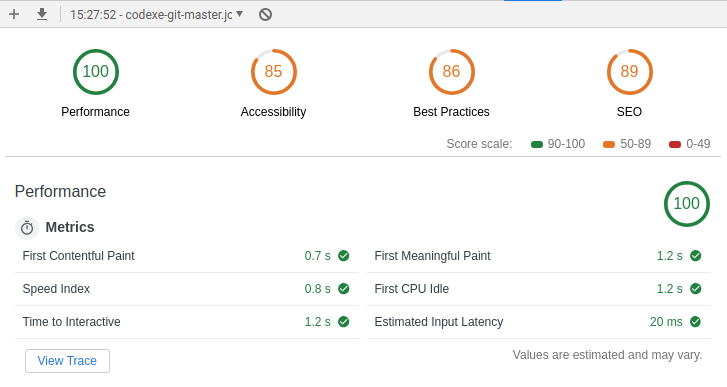
\includegraphics[scale=0.5]{res/lighthouse_audit_deployed.png}
    \caption{Lighthouse audit of deployed application}
    \label{deployed-lighthouse}
\end{figure}

The figure above shows some excellent results for the different measurements. Performance being 100 is particularly notable as most of Google's own products don't meet that high. This performance result is due to how Next.js packages the application for deployment which converts all of the React layout code into normal HTML, CSS which is very fast to render. It also isolates each page into what they call a \textit{lambda} function which means that the pages aren't always running and instead will be loaded on demand. This means there's no resource wastage from a server running 24 hours a day. The different metrics are shown at the bottom of the figure with extremely fast response times. It is worth mentioning again that this is a deployed system and is not running locally or hosted on the same LAN.

The accessibility score is only 85 as the code editor's theme has the green of the comment which has low contrast compared to the dark background, there is also an issue in the bullet point list of site features as screen readers will announce the globe images when really they shouldn't be noted. This can be fixed with an \texttt{aria-hidden} attribute on the element which will tell screen readers to ignore it. 

The best practices score is due to errors being logged in the console. As only the frontend is currently deployed, the WebSocket fails to connect which results in errors logged to the console. This will be resolved once the backend of the application is deployed. 

The SEO score is due to there not being a meta description of the website in the \texttt{<head>} which is what provides search engines with their summary of the website. This is very easy to resolve. 

\subsection{Docker Stats}

A number of tests were performed while visually observing the running of the \texttt{docker stats} command which provides real time usage on CPU, memory, I/O and more. It is worth noting before observing the results that while the usage can say 0\% that does not mean that 0\% of the CPU is being occupied by the container as there is a base level allocation of usage that, while may not be consumed, is still unavailable to other processes. This is mentioned in \cite{docker-perf}.

All tests were done 5 times and an average was taken.

%TODO: put processing power of CPU here somewhere

\begin{table}[h!]
    \centering
    \begin{tabulary}{\textwidth}{L|C|C}
        \textbf{Operation} & \textbf{CPU Usage (\%)} & \textbf{RAM Usage (MiB)}\\
        \hline
        Server Started & Server Idling at 0.1 & Server Idling at 195.7\\
        \hline
        Container Started & No change in server. New container 'Modi' idling at 0. & Server idling at 196.3. Modi idling at 1.234\\
        \hline
        Counting to 50 million & Server jumps to 0.66. Modi peaks at 55. & No change in server. Modi peaked at 2.55. Modi idles higher post execution at 2.023\\
        \hline
        Connecting the Terminal & Server jumps to 1. No change in Modi. & No changes in either container.\\
        \hline
        Typing in the Terminal & Server peaks at 3.88. Modi peaks at 0.35. & No changes in either container.\\
        \hline
        Opening a file & Server peaks at 0.7. Modi peaks at 4.3. & No changes in either container.\\
        \hline
        Opening a Python Exercise & Server doesn't change. Modi pauses and idles at 0. Python container idles at 0. & No change in server memory use. Modi idles at 2.023 Python container idles at 5.625.\\
        \hline
        Counting to 50 million in exercise & Server doesn't change. Python peaks at 50. & Server doesn't change. Python peaks at 8.\\
        \hline
        Opening a new tab & Server behaves the same as opening container. New container idles with 0. & No change to server. Modi remains idling at 2.023. New container idles at 0.956.
    \end{tabulary}
\end{table}

\subsubsection{Observations}

Node.js idles with relatively high memory consumption but incredibly low CPU usage. 

Containers will take up as much CPU as they can when they are doing intense computation.

Memory consumption for containers never goes higher than 8MiB at peak and never idles higher than 5.625MiB.

Usage scales dynamically in all aspects.

Biggest potential problems is will many containers trying to do intense computation at once.

\section{Security}

% Pen testing

Security is a big concern with a system where users have the ability to not only execute code on a remote machine but also have access to the shell of a container that will be deployed to the same space that the entire backend will be. Despite containers providing huge advantages speed/size wise over hypervisor powered virtual machines, from a security perspective there is a large problem. The containers are running on the kernel of the machine that the container provisioning engine is running on so if a user is able to exploit a kernel bug, it means that they can break out of the container and start changing things in the shell of the machine hosting the entire system. This would be terrible if the attacker has malicious intent.

A lot of kernel exploits are only possible with root access so the first step to securing the containers is making sure that the user account that the users are logged into is not the normal docker root user. This is briefly discussed in Section \ref{impl-alloc} with the Dockerfile that creates the \textit{damien} user which is what users are occupying while they're on the system. Inside this normal user account access to sensitive information is well secured, a lot of commands that can be used maliciously are locked, the ability to install more software (like cracking tools and fingerprinting tools) is not available. One potential issue is that some of the default binaries installed which are usable, even though they aren't meant for malicious purposes could be exploited to do something malicious. The \texttt{wget} package is an example of this as on the surface it's a tool for downloading a web page but it could be used to download scripts online and then so long as they're in the users home folder they will be able to execute them. 

More tools that could help prevent exploitation of the service that this project is providing would be a long running watcher which checks to see that there aren't any containers operating at 100\% CPU usage for too long. This type of usage could indicate that someone is trying to break the containers/the overall system. Usage limits and tracking would aid in detecting this behaviour and providing a warning to users that this type of activity could result in being black listed from the system.

Preventing security issues is an endless task however a new tool from Google is proving effective at mitigating the risk of using containers as remote environments. gVisor \cite{gvisor} is compliant with the Open Container Initiative and works as a drop in runtime for the \texttt{runc} runtime that Docker uses by default and provides a small layer of security on top similar to how a traditional hypervisor provides security.

\begin{figure}[h!]
    \centering
    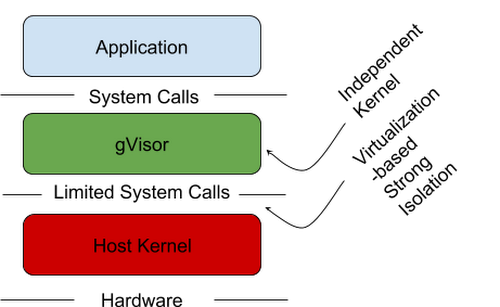
\includegraphics[scale=0.5]{res/gvisor.PNG}
    \caption{gVisor Runtime Architecture \cite{gvisor-info}}
    \label{fig:gvisor}
\end{figure}

Shown in the article \cite{gvisor-info} simply replacing the \texttt{runc} runtime with the gVisor based \texttt{runsc} means that a specific kernel exploit no longer works in containers. This type of technology is inevitable as more huge industry giants adopt containerisation and provides an optimistic view of how using containers can be both well performing and secure.

\pagebreak
